%===================================== CHAP 3 =================================



\chapter{Object Detection}
The problem of detecting objects in an image is harder than classifying an image only containing one object. In object detection the goal is both to classify objects and locate the exact location of the object in the image. That makes the problem twofold, first we need to find subregions in the image, and then we need to classify them. Since the latter part of the problem has been solved by CNNs, the part that remains is to find these subregions. 

\begin{figure}[h!]
    \centering
    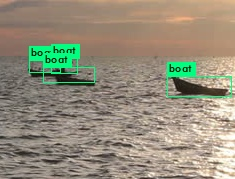
\includegraphics[scale=0.8]{images/predictions2.jpg}
    \caption{Detected boats.}
    \label{fig:boat_detection}
\end{figure}


\section{Sliding Window (OverFeat)}
The most straightforward solution to find subregions in an image is to use a sliding window, and OverFeat \citep{Sermanet2013} is a method that applies this technique. The sliding window is a window that convolves over the image, like the filters explained in chapter \ref{sec:conv}, and looks at small regions of the image one at a time. This region is then passed through a classification network to determine if this region contains an object of interest. If the classification network returns a high confidence score, OverFeat considers it as an object. 

\vspace{3mm}

The problem with this approach is that it is very computationally exhaustive, and it is also not scale invariant, meaning we have to try several different scales for the sliding windows to be able to detect objects of different sizes. This means that OverFeat has to classify very many subregions, and is therefore not a good option for real-time systems.


\section{R-CNN - Regions with Convolutional Neural Networks }
R-CNN (Regions with Convolutional Neural Networks  \citep{R-CNN}), attacks the problem differently than OverFeat. Instead of trying arbitrary subregions, they propose a solution using the Selective Search algorithm for region proposals.

\subsection{Selective Search }
The Selective Search algorithm \citep{SelSearch} groups adjacent pixels based on color, texture and intensity together and creates segmented pictures as shown in figure \ref{fig:sel_serach}. It is designed to have very high recall, meaning that it is accepted to suggest several false positives, as long as it gets all the true positives. Recall is explained further in chapter \ref{sec:prec_rec}.

\vspace{3mm}

The Selective Search algorithm takes a segmented image as initial input and performs the following steps:
\begin{enumerate}
  \item Add bounding boxes corresponding to segmented parts to the list of region proposals. This means that regions with the same color (as shown in figure \ref{fig:sel_serach}) will be grouped together in a bounding box. A bounding box is a rectangular box that surrounds a potential object.
  \item Group adjacent segments based on similarity.
  \item Go to step 1.
\end{enumerate}

\begin{figure}[h!]
    \centering
    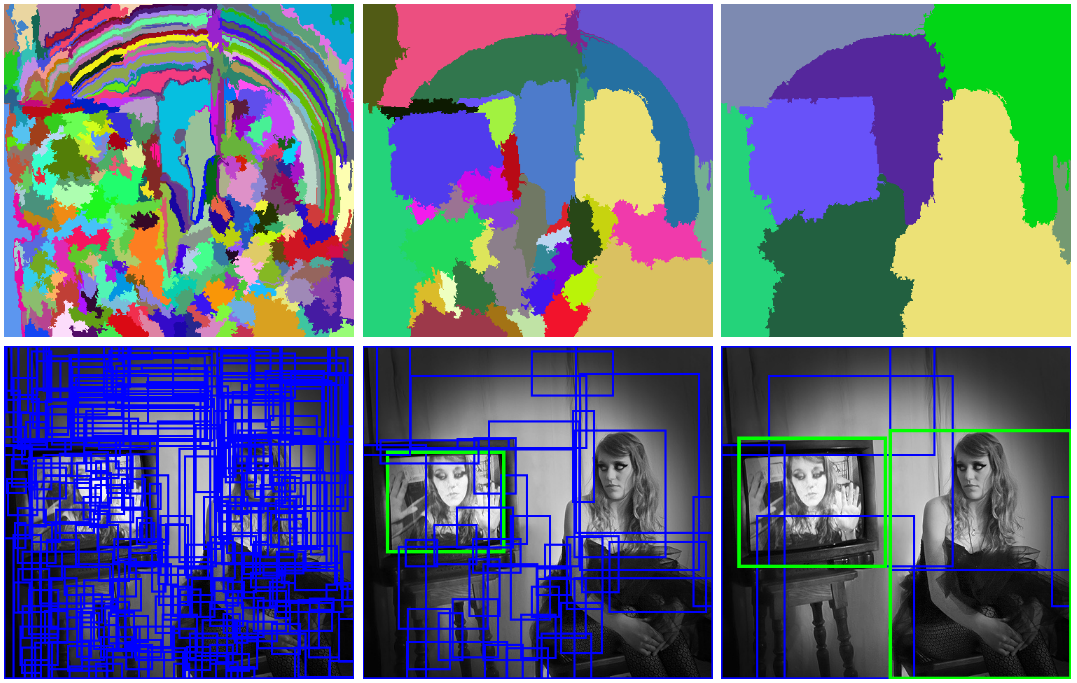
\includegraphics[scale=0.5]{fig/sel_search.png}
    \caption{Segmented regions shown in top row, and bounding boxes returned shown in bottom row. This shows why different scales of segmentation is important, since bigger objects are only detected when the image is less segmented. Image from \citep{SelSearch}.}
    \label{fig:sel_serach}
\end{figure}





\newpage

After Selective search has created the region proposals, R-CNN inputs these to a convolutional neural network. The CNN classifies all the region proposals, and if the confidence of the classification is high, the bounding box with its class is outputted from the algorithm. 


\section{Fast R-CNN}

Two years after the release of R-CNN, Fast R-CNN  \citep{FastR-CNN} was released by the same author. In this time he had discovered two drawbacks with R-CNN, and found solutions to the problems. 

\begin{enumerate}
    \item R-CNN consists of three different models that all have to be trained. In addition to the CNN, R-CNN consists of a Support Vector Machine (SVM) for classification, and a bounding box regressor, which tightens the bounding boxes around detected objects. Since R-CNN consists of three parts that are trained independently, it makes it harder to train the network as a whole. This is because they are optimizing for themselves and not for the entire system. 
    \item The CNN has to run once for every region proposal from Selective Search. Since Selective Search is designed to have a very high recall, this ends up being a bottleneck. 
\end{enumerate}

\subsubsection{Solution to Problem 1}
Instead of training the three parts of the network individually, Fast R-CNN changed the structure in a way that let the whole system be trained together.

\subsubsection{Solution to Problem 2}
Instead of calculating the CNN features for every subregion of the image, the CNN features for the entire image were calculated once. Then the features of every region were extracted from this feature map.



\section{Faster R-CNN }
The bottleneck in Fast R-CNN was the region proposals and the Selective Search algorithm. The idea behind Faster R-CNN \citep{FasterR-CNN} is that the region proposals should depend on the features calculated by the CNN. So instead of using Selective Search, we can use the feature maps outputted from the CNN. The feature maps are then inputted in a Region Proposal Network (RPN), which uses a sliding window over the CNN feature map, and outputs k potential bounding boxes and scores for how good these boxes are expected to be. These proposals are then fed into a the same classifier as used in Fast R-CNN. The difference between the two is just that the region proposals depend only on CNN features in Faster R-CNN, thus it bypasses the Selective Search algorithm.



\section{YOLO - You Only Look Once }
\label{sec:yolo}
What separates YOLO \citep{YOLOv1} \citep{YOLOv2} \citep{YOLOv3} from R-CNN methods is that YOLO only looks once at the picture, and there is only one network for the entire detection process. "We reframe object detection as a single regression problem, straight from image pixels to bounding box coordinates and class probabilities. Using our system, you only look once (YOLO) at an image to predict what objects are present and where they are." \citep{YOLOv1}. 
\vspace{0.5cm}

YOLO starts by dividing the input image into a SxS grid. The goal for each cell is to predict B bounding boxes, and confidence scores for these boxes. If an object has its center in a cell, that cell is responsible for detecting that object. The score of the box says how confident it is that the bounding box contains an object and how accurate it thinks the box is. 

\begin{equation}
    \text{Confidence score} = \text{P(Object)} \cdot \text{IoU}
\end{equation}

Where IoU is the \textit{Intersect over Union} between the predicted box and ground truth, shown in figure \ref{fig:IoU}. Ground truth is here a manually drawn box over a correct object in the image.


\begin{figure}[h!]
\centering
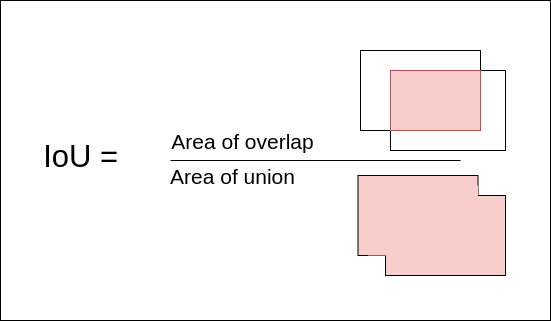
\includegraphics[scale=0.5]{fig/iou.png}
\caption{Intersect over Union}
\label{fig:IoU}
\end{figure}

Each grid cell also predicts C conditional class probabilities, which are conditional on that cell containing an object. P(Class$|$Object). For each cell, only one set of class probabilities is calculated. To get class specific scores for each bounding box we multiply these together. 

\begin{equation}
    \text{P(Class}|\text{Object)} \cdot \text{P(Object)} \cdot \text{IoU}
    \label{eq:yolo}
\end{equation}

This gives a value of how well the predicted box fits the object, and the probability of that class appearing in the box. When we have this value we can set a threshold, and only use the results that are probable as output. This is shown in figure \ref{fig:yolo_flow}.  

\begin{figure}[h!]
\centering
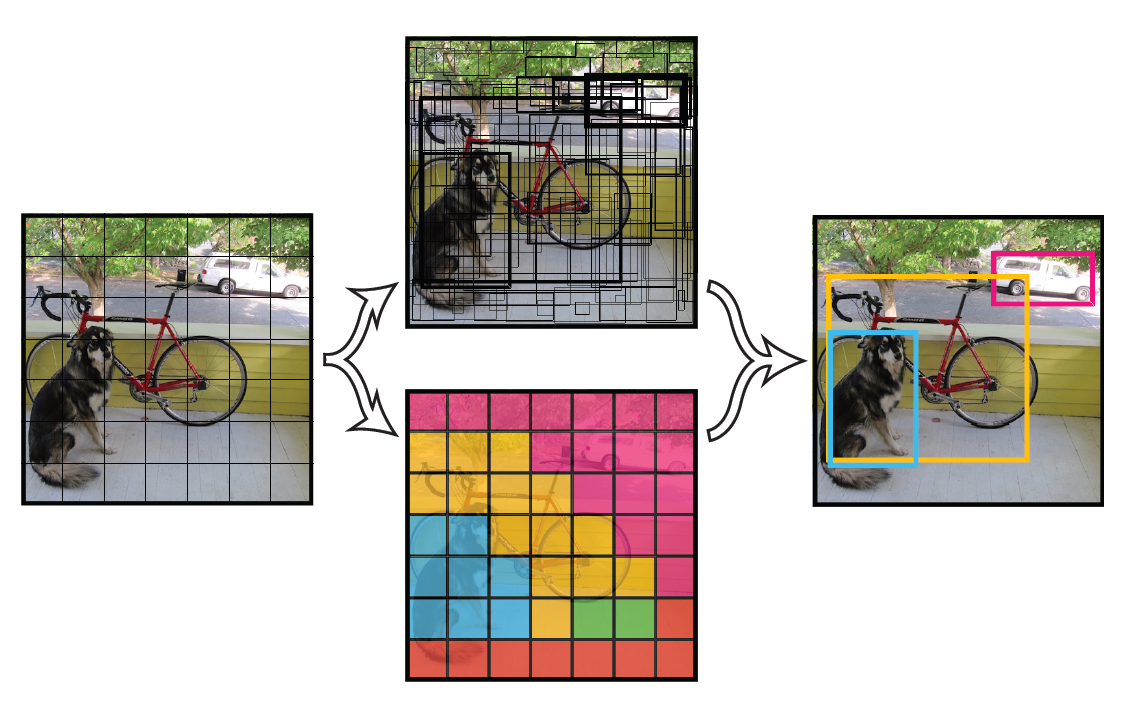
\includegraphics[scale=0.4]{images/YOLO_flow.png}
\caption{YOLO flow, Top image shows predicted bounding boxes, the thicker the line the higher the confidence score. The bottom picture shows the class probability map. These combined together gives the output image, (Equation \ref{eq:yolo}), image from \citep{YOLOv1}}
\label{fig:yolo_flow}
\end{figure}

%\subsection{Limitations and possible solution}
%The way YOLO grids the input image has several advantages, but also comes with some drawbacks. As mentioned earlier, each cell can only predict one class, and also predicts a limited amount of bounding boxes. Hence, YOLO struggles with small objects that lie close together. I tried running YOLO on some images gotten online, and it seems like this could be a problem for boats that are far away. In figure \ref{fig:pred} one of the boats in the top right corner is not detected. But if i zoom in on that part of the image, and run it through the same network I get the results shown in figure \ref{fig:pred2}. Here are the bounding boxes more accurate, and it actually detects a man standing on the foremost boat as well. YOLO does not seem to have a problem with the lowered resolution. 


\newpage

\section{SSD - Single shot Multibox Detector}
The Single Shot Multibox Detector works in a similar fashion as YOLO compared to Faster R-CNN. SSD does not use a region proposal network, but as YOLO, it discards the proposal generation step and does all the computation in a single network. A difference between YOLO and SSD is that SSD uses different aspect ratios and scales when it grids the input image, which makes it easier to handle objects with different sizes. By circumventing the proposal generation step SSD saves computational time and runs at a frame rate six to eight times higher than Faster R-CNN with similar accuracy, according to \citep{SSD}. 

\begin{figure}[h!]
    \centering
    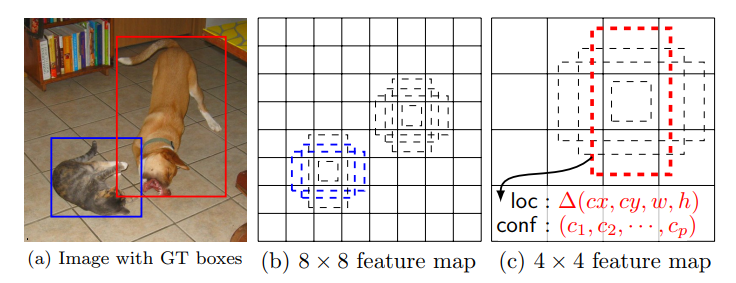
\includegraphics[scale=0.5]{images/ssd_detection.png}
    \caption{SSD training process, image from \citep{SSD}}
    \label{fig:ssd_training}
\end{figure}

Figure \ref{fig:ssd_training} shows how SSD detects objects with different sizes using different aspect ratios on the feature map. Each cell in the feature maps tries different \textit{anchors}, that are proprtional to the cell size. The \textit{anchors} are the default boxes shown with dotted lines in figure \ref{fig:ssd_training}. The smallest ground truth object in the image was found in the 8 by 8 grid, while the bigger object is found using the 4 by 4 grid, illustrating how different grid sizes detects objects of different size. The anchors for each cell are run through a classifier which gives a confidence score, if multiple boxes predict the same class and has an \textit{intersect over union} of more than 0.5 the bounding box that has the highest confidence score is chosen. This process is called \textit{non-maximum suppression}.


\section{Object Detection in Maritime Environments}
\label{sec:obj_det}


\subsection{General Purpose Object Detectors}
In recent years several deep learning based object detectors have come along. These are trained on general datasets like VOC \citep{Everingham2012}\citep{Everingham2007}, ImageNet \citep{Imagenet} and COCO \citep{COCO},  and can be further trained for specific cases, such as object detection in maritime environments. These methods can be separated into two groups 

\begin{enumerate}
\item Region proposal based methods, which include R-CNN \citep{R-CNN}, Fast R-CNN \citep{FastR-CNN}, Faster R-CNN \citep{FasterR-CNN}, R-FCN \citep{R-FCN}, Mask R-CNN \citep{MaskRCNN}
\item Regression/classification based methods, which include SSD \citep{SSD}, YOLO \citep{YOLOv1} \citep{YOLOv2} \citep{YOLOv3}, MultiBox \citep{Multibox}, RetinaNet \citep{Retinanet}
\end{enumerate}




\subsection{Background Modelling}

Background modelling methods aims to model the background in order to detect foreground or moving objects. In \citep{BackgroundWaveletSubstract} the authors propose a method for detecting boats using dynamic background modeling and shadow suppression in order to detect boats. Other articles dealing with port surveillance with object detection are \citep{SeeCoast}, \citep{Pires2010}. \citep{Tran2016} uses background substraction to detect moving boats, and saliency detection to detect non-moving boats. These results are finally fused to generate the detected boats in the scene. 

\subsection{Appearance Based Methods}
Appearance based methods seeks to model the vessels appearance, and to classify it. \citep{HOGdetection} uses HOG-like features and background substraction together to detect boats. \citep{HAARdetection} detects boats from a rotatable camera using HAAR-like features. In \citep{Wedel2007} video is used to verify obstacles, and find obstacle boundaries, to supplement radar signals. \citep{RIBDetection} detects small, fast moving RIB boats that are hard for radars to detect and track.  

\vspace{3mm}

\citep{SSD_detection2018} aims to develop a real-time detection and tracking system for surveillance cameras in harbours. They have gathered a dataset of 48,966 images containing 70,513 ships from several viewpoints, and trained a detector based on SSD \citep{SSD} to perform detection. 


\subsection{Other relevant research}

In \citep{KITTI}, the KITTI Vision Benchmark Suite is presented as "In this paper, we take advantage
of our autonomous driving platform to develop novel challenging
benchmarks for the tasks of stereo, optical flow, visual
odometry / SLAM and 3D object detection."  KITTI is a dataset that can be used to benchmark detection algorithms for autonomous cars.

\citep{Sun2006} gives a thorough review of detection methods used for autonomous cars. 

\vspace{3mm}

In \citep{Hog1} and \citep{Hog2}, the author tries to detect small boats in satellite images with very high resolution. Large parts of the image does not contain boats, while smaller sub frames contains many boats. His solution is to find these sub frames by using edge detection methods, and then run YOLO. This problem is to some degree relatable to the problem of detecting boats from ships. However, satellite images have much less background noise, e.g. from waves. Running the same edge detection algorithms on images taken at sea level returns a lot of noise, and the result is therefore hard to replicate with the same success. 

\vspace{3mm}

Summed up there are many different approaches to the problem of detecting boats in images. A problem with these articles is that even though they give performance metrics on their dataset, there is no way of concluding that their solution will perform as well in other environments. \citep{SSD_detection2018} for instance, trains an SSD detector for detection of boats, it discusses how the detector performs on boats of different sizes, and it also mentions that it performs worse in "difficult situations such as low light, very small ships and clutter from in-harbor ships" \citep{SSD_detection2018}. Still, the only performance statistic provided is how well the detector performs on the dataset as a whole. This gives a good indication that SSD can be a good option. However, an object detector meant to supplement other sensors on an autonomous ship should have known performance statistics in different environments and under different circumstances to be able to trust it in a real scenario. 

\vspace{3mm}

The work in this project addresses this problem by making it easy to test and train different object detectors on different data. This way different detectors can be benchmarked against eachother, while trained and tested on the same data. During this project YOLO and SSD has been chosen as a starting point in this research, training the detectors on data where boats are moored, at sea, far away and close. They are also trained and tested on images captured in areas where it is desireable that it will perform well.





\cleardoublepage